\documentclass[11pt]{report}
\usepackage[utf8]{inputenc}	% Para caracteres en español
\usepackage{amsmath,amsthm,amsfonts,amssymb,amscd}
\usepackage{multirow,booktabs}
\usepackage[table]{xcolor}
\usepackage{fullpage}
\usepackage{lastpage}
\usepackage{enumitem}
\usepackage{fancyhdr}
\usepackage{mathrsfs}
\usepackage{wrapfig}
\usepackage{setspace}
\usepackage{hyperref}
\usepackage{calc}
\usepackage{multicol}
\usepackage{cancel}
\usepackage[retainorgcmds]{IEEEtrantools}
\usepackage[margin=3cm]{geometry}
\usepackage{amsmath}
\newlength{\tabcont}
\setlength{\parindent}{0.0in}
\setlength{\parskip}{0.05in}
\usepackage{empheq}
\usepackage{framed}
\usepackage[most]{tcolorbox}
\usepackage{xcolor}
\colorlet{shadecolor}{orange!15}
\parindent 0in
\parskip 12pt
\geometry{margin=1in, headsep=0.25in}
\theoremstyle{definition}
\usepackage{pdfpages}
\newtheorem{defn}{Definition}
\newtheorem{reg}{Rule}
\newtheorem{exer}{Exercise}
\newtheorem{note}{Note}
\usepackage{fancyhdr}\usepackage{xcolor}\usepackage{amsmath}\usepackage{amssymb}\pagestyle{fancy}\rhead{}
\newtheorem{theorem}{Theorem}[subsection]
\theoremstyle{definition}
\newtheorem{definition}[theorem]{Definiton}
\newtheorem{example}[theorem]{Example}
\newtheorem{corollary}[theorem]{Corollary}
\newtheorem{lemma}[theorem]{Lemma}
\title{Chapter 9 Review Notes}
\begin{document}
\thispagestyle{empty}
{\LARGE \bf ECE 253 Lecture Notes}\\
{\large Hei Shing Cheung}\\
Digital and Computer Systems, Fall 2025 \hfill ECE253\\
\\
The up-to-date version of this document can be found at \url{https://github.com/HaysonC/skulenotes}\\

\chapter{Digital Circuits that Compute, Store, and Control}
\begin{shaded}
\section*{Introduction}
\paragraph{Layers of Computation} In hardware, we have the following layers of abstraction:
\begin{itemize}
    \item Computation
    \item Adders 
    \item Logic Gates
    \item Transistors
    \item Silicon
\end{itemize}
In this course, we will focus on the first three layers, on top of the logic gate level.


\paragraph{Layer of abstraction} At this course, for the digital systems part, we would start from understanding logic gates, all the way to understanding computer architecture, with each level of abstraction hiding the details of the lower level.

\section{Hierarchy, Modularity, and Regularity}

\begin{definition}[Hierarchy]
    The division of system into a set of modules, then further subdividing each module into smaller modules, and so on, until pieces are \textit{easy} to understand.    
\end{definition}

\begin{definition}[Modularity]
    The design principle that modules have well-defined functions and interfaces so they connect easily without unintended side effects.
\end{definition}

\begin{definition}[Regularity]
    The uniformality of modules, such that the reusability of common modules reduces the number of distinct modules to be designed.
\end{definition}

\subsection{Digital Logic Gates}
Logic gates are made out of transistors:
\begin{definition}[Transistor]
    A transistor is a 3-terminal device behaving as a switch. When the voltage on the terminal is HI, the switch is closed, and when the voltage is LO, the switch is open.
\end{definition}

\paragraph{Factors Affecting Speed of Digital Circuits}
\begin{itemize}
    \item \textbf{Transistors and Electrons take time to switch.} A transistor (State of the Art) takes 2-3 picoseconds to switch. Gates takes 40 ps and an 8-bit adder takes 300 ps.
    \item \textbf{Wires take time to propagate signals.} Signals travel at approximately 2/3 the speed of light in a vacuum, which is about 200,000 kilometers per second in a typical silicon wire.
    \item \textbf{Capacitance} There would be RCL circuits formed by the wires and transistors, which would cause delay.
\end{itemize}

\end{shaded}

% ===================== PART A: DIGITAL LOGIC FOUNDATIONS =====================
\section{Digital Logic Foundations}
% Representation and arithmetic first, then devices and gates, then algebra/minimization
% --- Representation ---
\subsection{Number Systems}
\begin{definition}[Number System]
    A number system is a way of representing numbers using a set of symbols (digits) and a base (radix). The base determines the number of unique digits that can be used in the number system.
\end{definition}

\paragraph{Common Number Systems} You should be familiar with the following number systems:
\begin{itemize}
    \item Decimal (Base 10): Digits 0-9
    \item Binary (Base 2): Digits 0-1
    \item Hexadecimal (Base 16): Digits 0-9, A-F
\end{itemize}

In computer systems, we use binary to represent information, and we would often use hexadecimal to represent binary numbers in a more compact way - a group of 4 bits (a nibble) can be represented by a single hexadecimal digit.

\begin{example}[Binary, Decimal, and Hexadecimal Numbers]
    Below is a table showing the conversion of binary numbers to decimal numbers, along with their hexadecimal representation.
    \begin{table}[h!]
        \centering
        \begin{tabular}{|c|c|c|}
            \hline
            Binary & Decimal & Hexadecimal \\
            \hline
            0000 & 0 & 0 \\
            0001 & 1 & 1 \\
            0010 & 2 & 2 \\
            0011 & 3 & 3 \\
            0100 & 4 & 4 \\
            0101 & 5 & 5 \\
            0110 & 6 & 6 \\
            0111 & 7 & 7 \\
            1000 & 8 & 8 \\
            1001 & 9 & 9 \\
            1010 & 10 & A \\
            1011 & 11 & B \\
            1100 & 12 & C \\
            1101 & 13 & D \\
            1110 & 14 & E \\
            1111 & 15 & F \\
            \hline
        \end{tabular}
        \caption{Binary to Decimal and Hexadecimal Conversion}
    \end{table}
    
\end{example}
\begin{example}[Decimal to Binary Conversion]
    To convert a decimal number to binary, we can use the method of successive division by 2. For example, to convert the decimal number 437 to binary:
    \begin{align*}
        437 \div 2 &= 218 & \text{remainder 1} \\
        218 \div 2 &= 109 & \text{remainder 0} \\
        109 \div 2 &= 54 & \text{remainder 1} \\
        54 \div 2 &= 27 & \text{remainder 0} \\
        27 \div 2 &= 13 & \text{remainder 1} \\
        13 \div 2 &= 6 & \text{remainder 1} \\
        6 \div 2 &= 3 & \text{remainder 0} \\
        3 \div 2 &= 1 & \text{remainder 1} \\
        1 \div 2 &= 0 & \text{remainder 1}
    \end{align*}
    Reading the remainders from bottom to top, we get the binary representation of 437
\end{example}

\begin{example}
    To convert (512000)$_{10}$ to binary, we recognize that $512000 = 2^9 \times 1000$. We know that $2^9 = 512$ and $1000_{10} = 1111101000_2$ (by method outlined above). Therefore, we can shift the binary representation of 1000 left by 9 bits to get the binary representation of 512000:
    \[(512000)_{10} = (1111101000000000000)_2\]
\end{example}

\paragraph{Note} An alternative method is to devide by powers of 2.
\begin{shaded}
    \textbf{Fractional Numbers. } To represent fractional numbers in binary, we can use the method of successive multiplication by 2 (fixed point representation). Or we can use floating point representation, which is similar to scientific notation in decimal. 
\end{shaded}
\subsection{Binary Arithmetic and Logic}
\paragraph{Binary Arithmetic} Binary arithmetic is similar to decimal arithmetic, but it only uses two digits (0 and 1). Addition is associated with a sum and carry.

\paragraph{Binary Addition} The rules for binary addition are as follows: \\
\begin{table}[h!]
    \centering
    \begin{tabular}{|c|c|c|}
        \hline
        A & B & Sum, Carry \\
        \hline
        0 & 0 & 0, 0 \\
        0 & 1 & 1, 0 \\
        1 & 0 & 1, 0 \\
        1 & 1 & 0, 1 \\
        \hline
    \end{tabular}
    \caption{Binary Addition}
\end{table}

This could be summerize as the following logic:
\begin{equation}
    \text{Sum} = A \oplus B, \quad \text{Carry} = A \cdot B
\end{equation}
\paragraph{Binary Subtraction} The rules for binary subtraction are defined using the addition of negative numbers (2's complement):

\begin{definition}[Least Significant Bit (LSB) and Most Significant Bit (MSB)]
    The least significant bit (LSB) is the rightmost bit in a binary number, while the most significant bit (MSB) is the leftmost bit.`'
    
\end{definition}
\begin{definition}[2's Complement]
    The 2's complement of a binary number is obtained by inverting all the bits (1's complement) and adding 1 to the least significant bit (LSB).
\end{definition}

\begin{example}[Number Inversion]
    To find the 2's complement of the binary number (10110010)$_2$:
    \begin{enumerate}
        \item Invert all the bits: (01001101)$_2$
        \item Add 1 to the LSB: 
        \[
        \begin{array}{c}
        \quad 01001101 \\
        +\, 00000001 \\
        \hline
        \quad 01001110 \\
        \end{array}
        \]
    \end{enumerate}
    Therefore, the 2's complement of (10110010)$_2$ is (01001110)$_2$.
\end{example}

\begin{definition}[Logic Function]
    A logic function $L: \{0,1\}^n \rightarrow \{0,1\}$ is a mathematical function that takes $n$ binary inputs and produces a single binary output based on a set of rules.
\end{definition}

\begin{definition}[Truth Table]
    A truth table is a tabular representation of a logic function that lists all possible combinations of input values and their corresponding output values.
    
\end{definition}

\begin{definition}[Boolean Algebra]
    Boolean algebra is a branch of algebra that deals with binary variables and logical operations. It provides a set of rules and properties for manipulating and simplifying logic functions. The specific rules and properties would be covered in later lectures.
\end{definition}
% --- Devices and gates ---
\subsection{Transistors as Switches}
\begin{definition}[Transistor]
    Transistor operates as a switch. The switch is open only when the gate is high. We denote the state of the gate as $x \in \{0,1\}$, where 0 is LO and 1 is HI. If input end of the switch is HI, the output end could be modeled by the logic function:
    $$
        L(x) = x
    $$
\end{definition}

\begin{example}[Serial Transistors]
    Consider two transistors connected in series, with the input end of the first transistor connected to HI. The output end of the second transistor can be modeled by the following truth table:
    \begin{table}[h!]
        \centering
        \begin{tabular}{|c|c|c|}
            \hline
            $x_1$ & $x_2$ & $L(x_1, x_2)$ \\
            \hline
            0 & 0 & 0 \\
            0 & 1 & 0 \\
            1 & 0 & 0 \\
            1 & 1 & 1 \\
            \hline
        \end{tabular}
        \caption{Truth Table for Two Transistors in Series}
        \label{tab:and_gate}
    \end{table}
    \\
    The logic function can be expressed as:
    $$
        L(x_1, x_2) = x_1 \cdot x_2
    $$
    where $\cdot$ denotes the AND operation.
\end{example}

\begin{example}[Parallel Transistors]
    Consider two transistors connected in parallel, with the input end of both transistors connected to HI. The output end can be modeled by the following truth table:
    \begin{table}[h!]
        \centering
        \begin{tabular}{|c|c|c|}
            \hline
            $x_1$ & $x_2$ & $L(x_1, x_2)$ \\
            \hline  
            0 & 0 & 0 \\
            0 & 1 & 1 \\
            1 & 0 & 1 \\
            1 & 1 & 1 \\
            \hline
        \end{tabular}
        \caption{Truth Table for Two Transistors in Parallel}
        \label{tab:or_gate}
    \end{table}
    \\
    The logic function can be expressed as:
    $$
        L(x_1, x_2) = x_1 + x_2
    $$
    where $+$ denotes the OR operation.
\end{example}

\begin{example}
    Consider a circuit with a transistor connected to LO and the output end connected to LO, The other ends of the output and the transistor are connected together to a HI (and a resistor). The output end of the circuit can be modeled by the following truth table:
    \begin{table}[h!]
        \centering
        \begin{tabular}{|c|c|}
            \hline
            $x$ & $L(x)$ \\
            \hline
            0 & 1 \\
            1 & 0 \\
            \hline
        \end{tabular}
        \caption{Truth Table for a Transistor Connected to LO}
        \label{tab:not_gate}
    \end{table}
    \\
    The logic function can be expressed as:
    $$
        L(x) = \overline{x}
    $$
    where $\overline{x}$ denotes the NOT operation.
\end{example}

\subsection{Basic Logic Gates}

\begin{definition}[AND Gate]
    An AND gate outputs 1 only if all inputs are 1. The truth table for a 2-input AND gate is shown in Table \ref{tab:and_gate}.
    \\
    The logic function for an AND gate with inputs $A$ and $B$ can be expressed as:
    $$
        L(A, B) = A \cdot B = AB 
    $$
    \textbf{Note} when no operator is present, it is assumed to be AND.

    The digital logic symbol for an AND gate is shown below:
    \begin{center}
        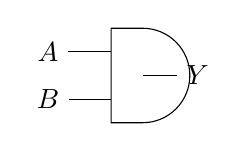
\begin{tikzpicture}[scale=1]
            % Simple custom AND gate to avoid reliance on gate shape anchors
            % Input nodes
            \node (A) at (-1,0.3) {$A$};
            \node (B) at (-1,-0.3) {$B$};
            % Wires to gate
            \draw (A.east) -- (-0.2,0.3);
            \draw (B.east) -- (-0.2,-0.3);
            % Gate body: rectangle on the left and semicircle on the right
            \draw (-0.2,0.6) -- (-0.2,-0.6) -- (0.2,-0.6) arc (-90:90:0.6) -- cycle;
            % Output
            \node (Y) at (0.9,0) {$Y$};
            \draw (0.6,0) -- (Y.west);
            \draw (0.2,0) -- (0.6,0);
        \end{tikzpicture}
    \end{center}    
\end{definition}

\begin{definition}[OR Gate]
    An OR gate outputs 1 if at least one input is 1. The truth table for a 2-input OR gate is shown in Table \ref{tab:or_gate}.
    \\
    The logic function for an OR gate with inputs $A$ and $B$ can be expressed as:
    $$
        L(A, B) = A + B
    $$
    The digital logic symbol for an OR gate is shown below:
    \begin{center}
        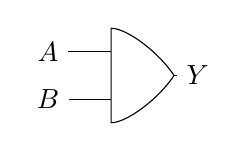
\begin{tikzpicture}[scale=1]
            % Simple custom OR gate to avoid reliance on gate shape anchors
            % Input nodes
            \node (A) at (-1,0.3) {$A$};
            \node (B) at (-1,-0.3) {$B$};
            % Wires to gate
            \draw (A.east) -- (-0.2,0.3);
            \draw (B.east) -- (-0.2,-0.3);
            % Gate body: curved shape
            \draw (-0.2,0.6) .. controls (0,0.6) and (0.4,0.3) .. (0.6,0) .. controls (0.4,-0.3) and (0,-0.6) .. (-0.2,-0.6) -- cycle;
            % Output
            \node (Y) at (0.9,0) {$Y$};
            \draw (0.6,0) -- (Y.west);
        \end{tikzpicture}
    \end{center}
\end{definition}    

\begin{definition}[NOT Gate]
    A NOT gate outputs the inverse of the input. The truth table for a NOT gate is shown in Table \ref{tab:not_gate}.
    \\
    The logic function for a NOT gate with input $A$ can be expressed as:
    $$
        L(A) = \overline{A}
    $$
    The digital logic symbol for a NOT gate is shown below:
    \begin{center}
        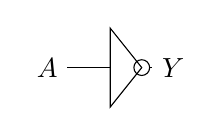
\begin{tikzpicture}[scale=1]
            % Input node
            \node (A) at (-1,0) {$A$};
            % Wire to gate
            \draw (A.east) -- (-0.2,0);
            % Gate body: triangle with circle at output
            \draw (-0.2,0.5) -- (0.2,0) -- (-0.2,-0.5) -- cycle;
            \draw (0.2,0) circle (0.1);
            % Output
            \node (Y) at (0.6,0) {$Y$};
            \draw (0.3,0) -- (Y.west);
        \end{tikzpicture}
    \end{center}
\end{definition}


\subsection{Additional Logic Gates}
\begin{example}[XOR Operation]
    We have two switches; when both switches are in the same state (both open or both closed), the output is 0. When the switches are in different states (one open and one closed), the output is 1. The truth table for this operation is shown below:
    \begin{table}[h!]
        \centering
        \begin{tabular}{|c|c|c|}      
            \hline
            $x_1$ & $x_2$ & $L(x_1, x_2)$ \\
            \hline
            0 & 0 & 0 \\
            0 & 1 & 1 \\
            1 & 0 & 1 \\
            1 & 1 & 0 \\
            \hline
        \end{tabular}
        \caption{Truth Table for XOR Operation}
        \label{tab:xor_gate}
    \end{table}
    \\
    The logic function can be expressed as:
    $$
        L(x_1, x_2) = x_1 \oplus x_2 = \overline{x_1}x_2 + x_1\overline{x_2}
    $$
    where $\oplus$ denotes the XOR operation.
\end{example}

\begin{definition}[XOR Gate]
    An XOR gate outputs 1 if the inputs are different. The truth table for a 2-input XOR gate is shown in Table \ref{tab:xor_gate}.
    \\
    The logic function for an XOR gate with inputs $A$ and $B$ can be expressed as:
    $$
        L(A, B) = A \oplus B = \overline{A}B + A\overline{B}
    $$
    where $\oplus$ denotes the XOR operation.
    The digital logic symbol for an XOR gate is shown below:
    \begin{center}
        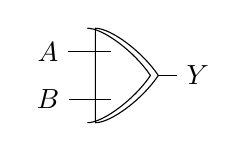
\begin{tikzpicture}[scale=1]
            % Input nodes
            \node (A) at (-1,0.3) {$A$};
            \node (B) at (-1,-0.3) {$B$};
            % Wires to gate
            \draw (A.east) -- (-0.2,0.3);
            \draw (B.east) -- (-0.2,-0.3);
            % Gate body: curved shape with extra curve on input side
            \draw (-0.4,0.6) .. controls (-0.2,0.6) and (0.2,0.3) .. (0.4,0) .. controls (0.2,-0.3) and (-0.2,-0.6) .. (-0.4,-0.6) -- cycle;
            \draw (-0.5,0.6) .. controls (-0.3,0.6) and (0.1,0.3) .. (0.3,0) .. controls (0.1,-0.3) and (-0.3,-0.6) .. (-0.5,-0.6);
            % Output
            \node (Y) at (0.9,0) {$Y$};
            \draw (0.4,0) -- (Y.west);
        \end{tikzpicture}
    \end{center}
\end{definition}


In addition, we have the following gates:
\begin{definition}[NAND Gate]
    A NAND gate outputs 0 only if all inputs are 1. The truth table for a 2-input NAND gate is as expected for the complement of AND.
    \\
    The logic function for a NAND gate with inputs $A$ and $B$ can be expressed as:
    $$
        L(A, B) = \overline{A \cdot B} = \overline{A} + \overline{B}
    $$
    The digital logic symbol for a NAND gate is shown below:
    \begin{center}
        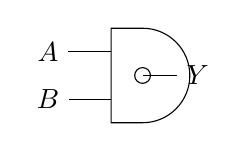
\begin{tikzpicture}[scale=1]
            % Input nodes
            \node (A) at (-1,0.3) {$A$};
            \node (B) at (-1,-0.3) {$B$};
            % Wires to gate
            \draw (A.east) -- (-0.2,0.3);
            \draw (B.east) -- (-0.2,-0.3);
            % Gate body: rectangle on the left and semicircle on the right with circle at output
            \draw (-0.2,0.6) -- (-0.2,-0.6) -- (0.2,-0.6) arc (-90:90:0.6) -- cycle;
            \draw (0.2,0) circle (0.1);
            % Output
            \node (Y) at (0.9,0) {$Y$};
            \draw (0.6,0) -- (Y.west);
            \draw (0.2,0) -- (0.6,0);
        \end{tikzpicture}
    \end{center}
\end{definition}

\begin{definition}[NOR Gate]
    A NOR gate outputs 1 only if all inputs are 0. The truth table for a 2-input NOR gate is the dual of the OR gate.
    \\
    The logic function for a NOR gate with inputs $A$ and $B$ can be expressed as:
    $$
        L(A, B) = \overline{A + B}
    $$
    % A minimal symbolic sketch could be added similar to OR with an inversion bubble; omitted for brevity.
\end{definition}

\begin{shaded}
    \textbf{NAND and NOR Gates are Cheaper} NAND gates and NOR gates are cheaper than AND and OR gates because they require fewer transistors to implement. A 2-input NAND gate can be implemented using 4 transistors, while a 2-input AND gate requires 6 transistors (4 for the NAND gate and 2 for the NOT gate). The same applies to NOR and OR gates.

    \textbf{NAND and NOR Gates are Universal (Functionally Complete)} Additionally, NAND and NOR gates are universal gates, meaning that any logic function can be implemented using only NAND or NOR gates. 
    
    This makes them more versatile and cost-effective for building complex digital circuits.
\end{shaded}


% --- Algebra and minimization ---
\paragraph{Commonly Used Logic Operators} Below is a table summarizing the commonly used logic operators:
\begin{table}[h!]
    \centering
    \begin{tabular}{|c|c|c|}
        \hline
        Operator & Symbol & Description \\
        \hline
    AND & $\cdot$ or adjacency & Outputs 1 if all inputs are 1 \\
    OR & $+$ & Outputs 1 if at least one input is 1 \\
    NOT & $\overline{x}$ or $x'$ or $\sim x$ & Outputs the logical negation of the input \\
    XOR & $\oplus$ & Outputs 1 if inputs are different \\
        NAND & $\overline{\cdot}$ & Outputs 0 if all inputs are 1 \\
        NOR & $\overline{+}$ & Outputs 0 if at least one input is 1 \\
        XNOR & $\overline{\oplus}$ & Outputs 1 if inputs are the same \\
        \hline
    \end{tabular}
    \caption{Commonly Used Logic Operators}
\end{table}

\subsection{Sum of Products (SOP) Form}
\begin{definition}[Literal]
    A literal is a variable or its negation. For example, $A$ and $\overline{A}$ are literals.  A literal can be either true or false, and it represents a single value in a logical expression.

\end{definition}

\begin{definition}[Product Term]
    A product term is a logical synonym for AND.
\end{definition}

\begin{definition}[Sum Term]
    A sum term is a logical synonym for OR.
\end{definition}

\begin{definition}[Sum of Products (SOP) Form]
    A logical expression is in sum of products (SOP) form if it is a sum of product terms. For example, the expression $AB + \overline{A}C + BC$ is in SOP form.
\end{definition}

\begin{definition}[Minterm]
    A product term that evaluates to one for exactly one row of the truth table is called a minterm.
\end{definition}
\begin{example}[Minterm]
    For a given truth table for $x_1, x_2, x_3$, the minterms are:
    \begin{table}[h!]
        \centering
        \begin{tabular}{|c|c|c|c|}
            \hline
            $x_1$ & $x_2$ & $x_3$ & Minterm \\
            \hline
            0 & 0 & 0 & $m_0 = \overline{x_1}\overline{x_2}\overline{x_3}$ \\
            0 & 0 & 1 & $m_1 = \overline{x_1}\overline{x_2}x_3$ \\
            0 & 1 & 0 & $m_2 = \overline{x_1}x_2\overline{x_3}$ \\
            0 & 1 & 1 & $m_3 = \overline{x_1}x_2x_3$ \\
            1 & 0 & 0 & $m_4 = x_1\overline{x_2}\overline{x_3}$ \\
            1 & 0 & 1 & $m_5 = x_1\overline{x_2}x_3$ \\
            1 & 1 & 0 & $m_6 = x_1x_2\overline{x_3}$ \\
            1 & 1 & 1 & $m_7 = x_1x_2x_3$ \\
            \hline
        \end{tabular}
        \caption{Minterms for 3 Variables}
        \label{tab:minterms}

    \end{table}
    \\
    Note that each minterm corresponds to a unique combination of input values that produces an output of 1. To create the minterm, you would try to make every literal one.

\end{example}

\begin{definition}[Canonical SOP Form]
    A logical expression is in canonical SOP form if it is a sum of minterms. 
\end{definition}

\subsection{Product of Sums (POS) Form}

\begin{definition}[Product of Sums (POS) Form]
    A logical expression is in product of sums (POS) form if it is a product of sum terms. For example, the expression $(A + B)(\overline{A} + C)(B + C)$ is in POS form.
\end{definition}


\begin{definition}[Maxterm]
    A sum term that evaluates to zero for exactly one row of the truth table is called a maxterm.
\end{definition}

\begin{example}[Maxterm]
    For a given truth table for $x_1, x_2, x_3$, the maxterms are:
    \begin{table}[h!]
        \centering
        \begin{tabular}{|c|c|c|c|}
            \hline
            $x_1$ & $x_2$ & $x_3$ & Maxterm \\
            \hline
            0 & 0 & 0 & $M_0 = (x_1 + x_2 + x_3)$ \\
            0 & 0 & 1 & $M_1 = (x_1 + x_2 + \overline{x_3})$ \\
            0 & 1 & 0 & $M_2 = (x_1 + \overline{x_2} + x_3)$ \\
            0 & 1 & 1 & $M_3 = (x_1 + \overline{x_2} + \overline{x_3})$ \\
            1 & 0 & 0 & $M_4 = (\overline{x_1} + x_2 + x_3)$ \\
            1 & 0 & 1 & $M_5 = (\overline{x_1} + x_2 + \overline{x_3})$ \\
            1 & 1 & 0 & $M_6 = (\overline{x_1} + \overline{x_2} + x_3)$ \\
            1 & 1 & 1 & $M_7 = (\overline{x_1} + \overline{x_2} + \overline{x_3})$ \\
            \hline
        \end{tabular}
        \caption{Maxterms for 3 Variables}
        \label{tab:maxterms}
    \end{table}
    \\
    Note that each maxterm corresponds to a unique combination of input values that produces an output of 0. To create the maxterm, you would try to make every literal zero.
\end{example}

\begin{definition}[Canonical POS Form]
    A logical expression is in canonical POS form if it is a product of maxterms.
\end{definition}

\begin{theorem}[Converting between Canonical Forms]
    Any logical expression can be converted from canonical SOP form to canonical POS form and vice versa. For $i \in \{0, 1, \ldots, 2^n - 1\}$ and $S \subseteq \{0, 1, \ldots, 2^n - 1\}$, we have:
    \[
        f(x_1, x_2, \ldots, x_n) = \sum_{i \in S} m_i = \prod_{i \notin S} M_i
    \]
\end{theorem}
\begin{example}
    We have the following converison:
    $$
        f(x_1, x_2, x_3) = m_1 + m_3 + m_5 + m_7 = M_0 M_2 M_4 M_6
    $$
\end{example}

\subsection{Boolean Algebra and Logic Minimization}
\begin{definition}[Boolean Algebra]
    Boolean algebra is a branch of algebra that deals with binary variables and logical operations. It is a effective means to describe logic circuits with a set of rules derived from the axioms of Boolean algebra.
\end{definition}

\begin{definition}[Axioms of Boolean Algebra]
    The axioms of Boolean algebra are a set of fundamental rules that govern the behavior of binary variables and logical operations. The number stems consist only of the set $\{0, 1\}$, with the following axioms:
    \begin{itemize}
        \item $0 \cdot 0 = 0$
        \item $1 \cdot 1 = 1$
        \item $0 \cdot A = 0 \cdot 1 = 1 \cdot 0 = 0$ for any $A$
        \item if $x=0$ then $\overline{x} = 1$
    \end{itemize}

    \textbf{Dual Form} We can also derive the following logical equivalences from the axioms:
    \begin{itemize}
        \item $A + 0 = A$
        \item $A + 1 = 1$
        \item $0 + 1 = 1 + 0 = 1$
        \item $A + \overline{A} = 1$
    \end{itemize}

    where $1$ is the multiplicative identity and $0$ is the additive identity.
\end{definition}

\paragraph{Rules derived from the Axioms of Boolean Algebra} The following rules can be derived from the axioms of Boolean algebra:
\begin{theorem}
\begin{itemize}
    \item $x \cdot 0 = 0$ (Annihilation)
    \item $x \cdot 1 = 1 \cdot x = x$ (Identity)
    \item $x \cdot \overline{x} = 0$ (Complementation)
    \item $x \cdot x = x$ (Idempotent)
    \item $x + 0 = 0 + x = x$ (Identity)
    \item $x + 1 = 1 + x = 1$ (Annihilation)
    \item $x + \overline{x} = 1$ (Complementation)
\end{itemize}
\end{theorem}

\begin{theorem}
The following identities can be derived from the axioms of Boolean algebra:
\begin{itemize}
    \item Commutative Laws:
    \begin{itemize}
        \item $A + B = B + A$
        \item $A \cdot B = B \cdot A$
    \end{itemize}
    \item Associative Laws:
    \begin{itemize}
        \item $A + (B + C) = (A + B) + C$
        \item $A \cdot (B \cdot C) = (A \cdot B) \cdot C$
    \end{itemize}
    \item Distributive Laws:
    \begin{itemize}
        \item $A \cdot (B + C) = A \cdot B + A \cdot C$
        \item $A + (B \cdot C) = (A + B) \cdot (A + C)$
    \end{itemize}
\end{itemize}
\end{theorem}
\begin{proof}
    By perfect induction. We can exhaustively check all possible values of $A$, $B$, and $C$ (0 or 1) to verify that both sides of each identity yield the same result.
\end{proof}

\begin{theorem}[Covering Theorem]
     The following is true:
    $$    
    x + xy = x
    $$
    and its dual:
    $$
    x(x + y) = x
    $$
\end{theorem}

\begin{theorem}[Combining Theorem]
    The following is true:
    $$
    xy + x\overline{y} = x
    $$
    and its dual:
    $$
    (x + y)(x + \overline{y}) = x
    $$
    
\end{theorem}

\begin{theorem}[De Morgan's Theorem]
    The following is true:
    $$
    \overline{xy} = \overline{x} + \overline{y}
    $$
    and its dual:
    $$
    \overline{x + y} = \overline{x} \cdot \overline{y}
    $$
\end{theorem}
\begin{proof}
    By direct proof. We have:
    \begin{align*}
        \overline{xy} &= \overline{x}\overline{y} + \overline{x}y + x\overline{y} \quad (\text{In Canonical SOP Form}) \\
        &= \overline{x}\overline{y} + \overline{x}y + x\overline{y} + x\overline{y} \quad (\text{Adding } x\overline{y} \text{ using $x + x = x$}) \\
        &= \overline{x}(\overline{y} + y) + \overline{y}(x + \overline{x}) \quad (\text{Using Distributive Law}) \\
        &= \overline{x} \cdot 1 + \overline{y} \cdot 1 \quad (\text{Using Complementation}) \\
        &= \overline{x} + \overline{y} \quad (\text{Using Identity})
    \end{align*}
\end{proof}

\begin{theorem}[Absorption / Redundancy Theorem]
    The following is true:
    $$
    x + \overline{x}y = x + y
    $$
    and its dual:
    $$
    x(\overline{x} + y) = xy
    $$
\end{theorem}
\begin{proof}
    By direct proof. We have:
    \begin{align*}
        x + \overline{x}y &= x + \overline{x}y + xy \quad (\text{Adding } xy \text{ using } x + xy = x) \\
        &= x(1 + y) + \overline{x}y \quad (\text{Using Distributive Law}) \\
        &= x \cdot 1 + \overline{x}y \quad (\text{Using Identity}) \\
        &= x + y \quad (\text{Using Combining Theorem})
    \end{align*}
\end{proof}

\paragraph{Summary of Important Theorems} The following table summarizes the important theorems/laws in Boolean algebra:
\begin{table}[h!]
    \centering
    \caption{Summary of Important Theorems/Laws in Boolean Algebra (original form and dual form)}
    \label{tab:boolean_algebra_summary}
    \begin{tabular}{|l|c|c|}
         \hline
            \textbf{Law / Theorem} & \textbf{Original Form(s)} & \textbf{Dual Form(s)} \\ \hline
            Commutative Law & $A + B = B + A$ & $A \cdot B = B \cdot A$ \\ \hline
            Associative Law & $A + (B + C) = (A + B) + C$ & $A \cdot (B \cdot C) = (A \cdot B) \cdot C$ \\ \hline
            Distributive Law & $A \cdot (B + C) = A \cdot B + A \cdot C$ & $A + (B \cdot C) = (A + B) \cdot (A + C)$ \\ \hline
            Identity Law & $A + 0 = A$ & $A \cdot 1 = A$ \\ \hline
            Null Law & $A + 1 = 1$ & $A \cdot 0 = 0$ \\ \hline
            Idempotent Law & $A + A = A$ & $A \cdot A = A$ \\ \hline
            Complement Law & $A + \overline{A} = 1$ & $A \cdot \overline{A} = 0$ \\ \hline
            Double Negation Law & $\overline{\overline{A}} = A$ & - \\ \hline
            De Morgan's Theorem & $\overline{A \cdot B} = \overline{A} + \overline{B}$ & $\overline{A + B} = \overline{A} \cdot \overline{B}$ \\ \hline
            Absorption / Redundancy Theorem & $A + \overline{A}B = A + B$ & $A(\overline{A} + B) = AB$ \\ \hline
            Combining Theorem & $AB + A\overline{B} = A$ & $(A + B)(A + \overline{B}) = A$ \\ \hline
            Covering Theorem & $A + AB = A$ & $A(A + B) = A$ \\ \hline  
    \end{tabular}
\end{table}
\newpage
\begin{shaded}
    \paragraph{Logic Minimization} The goal of logic minimization is to reduce the number of logic gates and inputs in a digital circuit while maintaining its functionality. This is important because it can lead to cost savings, improved performance, and reduced power consumption. Logic minimization can be achieved through various techniques, including Boolean algebra simplification, Karnaugh maps, and the Quine-McCluskey algorithm.
\end{shaded}

\begin{theorem}[Nand as SOP]
    And SOP circuit can be implemented using only NAND gates.
\end{theorem}

\begin{theorem}[Nor as POS]
    A POS circuit can be implemented using only NOR gates.
\end{theorem}

\begin{example}[Gumball Fact]
    Consider three sensors $s_0, s_1, s_2$ that detect defects in Gumballs. Those sensors are normally 0, but would be 1 if a defect is detected as follows:
    $$
        \begin{cases}
            s_0 = 1 & \text{if the Gumball is too small} \\
            s_1 = 1 & \text{if the Gumball is too big} \\
            s_2 = 1 & \text{if the Gumball is too light}
        \end{cases}
    $$
    We are to design a circuit that would output 1 if the Gumball is either too large or too small and too light. We can express canonical SOP form as:
    \begin{align*}
        L(s_0, s_1, s_2) &= m_3 + m_4 + m_5 + m_6 + m_7 \\ 
        &= \overline{s_0}s_1s_2 + s_2\overline{s_0}\overline{s_2} + s_0\overline{s_1}s_2 + s_0s_1\overline{s_2} + s_0s_1s_2 \\
        \intertext{Using the Combining Theorem}
        &= \overline{s_0}s_1s_2 + s_2\overline{s_0}\overline{s_2} + s_0s_2 + s_0s_1 \\
        \intertext{Using the Absorption Theorem}
        &= s_2\overline{s_0} + s_0s_2 + s_0s_1 \\
        \intertext{Using the Covering Theorem}
        &= s_2 + s_0s_1 
    \end{align*}
\end{example}

\begin{example}
    \textit{Derive a minimal POS expression for $f(x_1, x_2, x_3 = \prod M(0, 2, 4)$}
    \\
    We have:
    \begin{align*}
        f(x_1, x_2, x_3) &= M_0 M_2 M_4 \\
        &= (x_1 + x_2 + x_3)(x_1 + \overline{x_2} + x_3)(\overline{x_1} + x_2 + x_3) \\
    \intertext{Recognizing the combining theorem $(x+y)(x+\overline{y}) = x$}
        &= (x_1 + x_3)(x_2 + x_3)(\overline{x_1} + x_3) \\
        &= (x_1 + x_3)(x_2 + \overline{x_1} + x_3) \\
        &= (x_1 + x_3)(x_2 + x_3)
    \end{align*}   
\end{example}

\begin{theorem}[Transporting POS to SOP]
    A POS circuit can be implemented using only NAND gates. This is achieved by applying De Morgan's Theorem and the properties of NAND gates. We can use the trick $f = \overline{\overline{f}}$ to convert the POS expression into a form that can be implemented with NAND gates.
\end{theorem}
\begin{theorem}[Transporting SOP to POS]
    An SOP circuit can be implemented using only NOR gates. This is achieved by applying De Morgan's Theorem and the properties of NOR gates. We can use the trick $f = \overline{\overline{f}}$ to convert the SOP expression into a form that can be implemented with NOR gates.
\end{theorem}

\begin{example}
    \textit{Implement the function $f(x_1, x_2, x_3) = \sum m(1, 3, 5, 7)$ using only NAND gates.}
    \\
    We have:
    \begin{align*}
        f(x_1, x_2, x_3) &= m_1 + m_3 + m_5 + m_7 \\
        &= \overline{x_1}\overline{x_2}x_3 + \overline{x_1}x_2x_3 + x_1\overline{x_2}x_3 + x_1x_2x_3 \\
        &= x_3(\overline{x_1}\overline{x_2} + \overline{x_1}x_2 + x_1\overline{x_2} + x_1x_2) \\
        &= x_3(x_1 + x_2) \quad (\text{Using Combining Theorem}) \\
        &= \overline{\overline{x_3(x_1 + x_2)}} \quad (\text{Using } f = \overline{\overline{f}}) \\
        &= \overline{\overline{x_3} + \overline{x_1 + x_2}} \quad (\text{Using De Morgan's Theorem}) \\
        &= \overline{\overline{x_3} + (\overline{x_1} \cdot \overline{x_2})} \quad (\text{Using De Morgan's Theorem}) 
    \end{align*}    
\end{example}

% ===================== PART B: DESIGN METHODS AND HDL =====================
\section{Combinational Logic Circuits}

\begin{definition}[Combinational Logic Circuit]
    A combinational logic circuit is a digital circuit that implements a specific logic function using a combination of logic gates. The output of a combinational logic circuit depends only on the current inputs and not on any previous inputs or states. 
\end{definition}
\begin{definition}{Hardware Description Language (HDL)}
    A hardware description language (HDL) is a specialized programming language used to describe the structure, behavior, and operation of electronic circuits and systems. HDLs are used in the design and verification of digital systems, including integrated circuits (ICs) and field-programmable gate arrays (FPGAs). The two most commonly used HDLs are VHDL (VHSIC Hardware Description Language) and Verilog.
\end{definition}
\subsection{Introduction of Verilog}


\begin{definition}[Module]
    A module is a self-contained block of hardware that has inputs and outputs and an internal implementation (behavioral or structural). Modules are the unit of hierarchy in Verilog.
\end{definition}

\begin{example}[Module Block]
    A module block in Verilog is defined using the `module` keyword, followed by the module name and a list of input and output ports. For example:
    \begin{verbatim}
    module basic_logic(input logic a, b,
                       output logic w, x, y, z);
        assign w = a & b; // AND gate
        assign x = a | b; // OR gate
        assign y = ~a;    // NOT gate
        assign z = a ^ b; // XOR gate
    endmodule
    \end{verbatim}

    \textbf{Keywords} The keywords used in the module block are:
    \begin{itemize}
        \item \verb|assign|: Used to define continuous assignments for combinational logic.
        \item \verb|logic|: A type of variable that can hold binary values (0 or 1).
    \end{itemize}
\end{example}

\begin{definition}[Continuous Assignment]
    A continuous assignment is used to model combinational logic in Verilog. It is defined using the \verb|assign| keyword, followed by the output signal, the assignment operator `=`, and the logic expression. Continuous assignments are evaluated whenever any of the input signals change. That is, the output is considered instantaneously updated when the input changes (ignoring propagation delay).
\end{definition}
\subsection{Multiplexers (Mux)}
\begin{example}[2-1 Multiplexers (Mux)]
    \textit{Design a circuit that controls a light $f$ based on either two switches $x$ and $y$. The switch that control the light is determined by a control signal $s$. If $s = 0$, the light is controlled by switch $x$. If $s = 1$, the light is controlled by switch $y$.}
    \\
    We have the following truth table:

    \begin{table}[h!]
        \centering
        \begin{tabular}{|c|c|c|c|}
            \hline
            $s$ & $x$ & $y$ & $f$ \\
            \hline
            0 & 0 & 0 & 0 \\
            0 & 0 & 1 & 0 \\
            0 & 1 & 0 & 1 \\
            0 & 1 & 1 & 1 \\
            1 & 0 & 0 & 0 \\
            1 & 0 & 1 & 1 \\
            1 & 1 & 0 & 0 \\
            1 & 1 & 1 & 1 \\
            \hline
        \end{tabular}
        \caption{Truth Table for Mux}
        \label{tab:mux_truth_table}
    \end{table}
    
    From the truth table, we can derive the following canonical SOP expression:
    \begin{align*}
        f(s, x, y) &= m_2 + m_3 + m_5 + m_7 \\
        &= \overline{s}x\overline{y} + \overline{s}xy + s\overline{x}y + sxy \\
        &= \overline{s}x(\overline{y} + y) + sy(\overline{x} + x) \quad (\text{Using Distributive Law}) \\
        &= \overline{s}x \cdot 1 + sy \cdot 1 \quad (\text{Using Complementation}) \\
        &= \overline{s}x + sy \quad (\text{Using Identity})
    \end{align*}

    The verilog implementation is as follows:
    \begin{verbatim}
    module mux2to1(input logic x, y, s,
                   output logic f);
        assign f = (~s & x) | (s & y);
    endmodule
    \end{verbatim}
\end{example}

\paragraph{The Diagram of a Mux} is a trapezoid shown below:
\begin{center}
    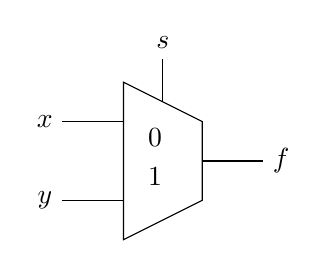
\begin{tikzpicture}[scale=1]
        % Input nodes
        \node (x) at (-2,0.5) {$x$};
        \node (y) at (-2,-0.5) {$y$};
        \node (s) at (-0.5,1.5) {$s$}; 
        % Wires to gate
        \draw (x.east) -- (-1,0.5);
        \draw (y.east) -- (-1,-0.5);
        \draw (s.south) -- (-0.5,0.75);
        % Gate body: trapezoid
        \draw (-1,1) -- (0,0.5) -- (0,-0.5) -- (-1,-1) -- cycle;
        % Output
        \node (f) at (1,0) {$f$};

        \node (0) at (-0.6,0.3) {0};
        \node (1) at (-0.6,-0.2) {1};
        \draw (0,0) -- (f.west);
    \end{tikzpicture}
\end{center}

\paragraph{4-1 Multiplexer (Mux)} A 4-1 Mux has 4 data inputs ($d_0, d_1, d_2, d_3$). The select signal would have two bit ($s_0, s_1$) to select one of the four data inputs to be outputted. In general, this is call a multibit signal, a.k.a a bus.
\begin{definition}[Bus]
    A bus is a bundle of signals. It is used to transfer data between different components of a digital system.
\end{definition}

\begin{example}[Verilog for a 2bit 2-1 Mux]
    The verilog implementation for a 2bit 2-1 Mux is as follows:
    \begin{verbatim}
    module mux2to1_2bit(input logic [1:0] x, y, // 2-bit inputs
                        input logic s,         // select signal
                        output logic [1:0] f); // 2-bit output
        assign f[0] = (~s & x[0]) | (s & y[0]); // LSB
        assign f[1] = (~s & x[1]) | (s & y[1]); // MSB
        // Alternatively, we can use the following single line:
        // assign f = s ? y : x; // If s=1, f=y; else f=x
    endmodule
    \end{verbatim}

    As we can see, we can initialize the datatype of a bus using the following syntax:
    \begin{verbatim}
    logic [n-1:0] bus_name; // n-bit bus
    \end{verbatim}
    
\end{example}

\subsection{Adders}
\begin{definition}[Half Adder]
    A half adder is a combinational logic circuit that performs the addition of two single-bit binary numbers. It has two inputs, typically denoted as $A$ and $B$, and two outputs: the sum ($S$) and the carry ($C$). The sum output represents the least significant bit of the addition, while the carry output represents any overflow that occurs when both inputs are 1. We start with the following truth table:
    \begin{table}[h!]
        \centering
        \begin{tabular}{|c|c|c|c|}
            \hline
            $A$ & $B$ & $S_1$ & $S_2$ \\
            \hline
            0 & 0 & 0 & 0 \\
            0 & 1 & 1 & 0 \\    
            1 & 0 & 1 & 0 \\
            1 & 1 & 0 & 1 \\
            \hline
        \end{tabular}
        \caption{Truth Table for Half Adder}
        \label{tab:half_adder_truth_table}
    \end{table}
    From the truth table, we can derive the following expressions using canonical SOP form:
    \begin{align*}
        S_0 &= m_1 + m_2 = \overline{A}B + A\overline{B} = A \oplus B \\
        S_1 &= m_3 = AB
    \end{align*}
    The Verilog implementation is as follows:
    \begin{verbatim}
    module half_adder(input logic A, B,
                      output logic [1:0] S);
        assign s[1] = a & b;
        assign s[0] = a ^ b;
    endmodule
    \end{verbatim}
\end{definition}

\begin{definition}[Full Adder]
    A full adder is a combinational logic circuit that performs the addition of three single-bit binary numbers: two significant bits and a carry-in bit. It has three inputs, we denote the signifcant bit as $A_i$ and $B_i$, and the carry-in bit as $C_i$, and two outputs: the sum ($S_i$) and the carry-out ($C_{i + 1}$). The sum output represents the least significant bit of the addition, while the carry-out output represents any overflow that occurs when the sum exceeds the value that can be represented by a single bit. We start with the following truth table:
    \begin{table}[h!]
        \centering
        \begin{tabular}{|c|c|c|c|c|}
            \hline
            $A_i$ & $B_i$ & $C_i$ & $S_i$ & $C_{i+1}$ \\
            \hline
            0 & 0 & 0 & 0 & 0 \\
            0 & 0 & 1 & 1 & 0 \\
            0 & 1 & 0 & 1 & 0 \\
            0 & 1 & 1 & 0 & 1 \\
            1 & 0 & 0 & 1 & 0 \\
            1 & 0 & 1 & 0 & 1 \\
            1 & 1 & 0 & 0 & 1 \\
            1 & 1 & 1 & 1 & 1 \\
            \hline
        \end{tabular}
        \caption{Truth Table for Full Adder}
        \label{tab:full_adder_truth_table}
    \end{table}
    From the truth table, we can derive the following expressions using canonical SOP form:
    \begin{align*}
        S_i &= m_1 + m_2 + m_4 + m_7 \\
            &= \overline{A_i}\overline{B_i}C_i + \overline{A_i}B_i\overline{C_i} + A_i\overline{B_i}\overline{C_i} + A_iB_iC_i \\
            &= A_i \oplus B_i \oplus C_i \\
        C_{i+1} &= m_3 + m_5 + m_6 + m_7 \\
                &= \overline{A_i}B_iC_i + A_i\overline{B_i}C_i + A_iB_i\overline{C_i} + A_iB_iC_i \\
    \intertext{Using the Distributive Law and A = A + A}
                &= B_iC_i(\overline{A_i} + A_i) + A_iB_i(\overline{C_i} + C_i) + A_iC_i(\overline{B_i} + B_i) \\
                &= A_iB_i + B_iC_i + A_iC_i
    \end{align*}
    The circuit diagram of a full adder is shown below:
    \begin{figure}[h!]
        \begin{circuitikz}
            \draw
            % gates 
            (0,0) node[xor port] (X1) {}
            (2,0) node[xor port] (X2) {}
            (1,-2) node[and port] (A1) {}
            (3,-2) node[and port] (A2) {}
            (2,-4) node[and port] (A3) {}
            (4,-4) node[or port] (O1) {} 
            (6,-4) node[or port] (O2) {};

            % connections
            \draw (X1.out) -- (X2.in 1);
            \draw (X2.out) -- ++(1,0) node[right] {$S_i$};

            % inputs
            \draw (X1.in 1) -- ++(-1,0) node[left] {$A_i$};
            \draw (X1.in 2) -- ++(-1,0) node[left] {$B_i$};
            \draw (X2.in 2) -- ++(-0.3,0) node[left] {$C_i$};

            % AND gate connections
            \draw (X1.in 1) |- (A1.in 1);
            \draw (X1.in 2) |- (A1.in 2);
            \draw (X1.in 2) |- (A2.in 1);
            \draw (X2.in 2) |- (A2.in 2);
            \draw (X1.in 1) |- (A3.in 1);
            \draw (X2.in 2) |- (A3.in 2);

            % OR gate connections
            \draw (A1.out) |- (O1.in 1);
            \draw (A2.out) |- (O1.in 2);
            \draw (A3.out) |- (O2.in 1);
            \draw (O1.out) |- (O2.in 2);
            \draw (O2.out) -- ++(1,0) node[right] {$C_{i+1}$}
        ;

        \end{circuitikz}
        \caption{Circuit Diagram of a Full Adder}
        \label{fig:full_adder_circuit}
        \centering 
    \end{figure}

    The Verilog implementation is as follows:
    \begin{verbatim}
    module full_adder(input logic A_i, B_i, C_i,
                      output logic S_i, C_i_plus_1)
        assign S_i = A_i ^ B_i ^ C_i;
        assign C_i_plus_1 = (A_i & B_i) | (B_i & C_i) | (A_i & C_i);
    endmodule
    \end{verbatim}
\end{definition}

\begin{definition}[Hierarchical Verilog Module]
    Hierarchical Verilog is a verilog module that instantiates other modules within it. This allows for the creation of complex designs by combining simpler modules.
\end{definition}
\begin{example}[3-bit Ripple Carry Adder]
    A 3-bit ripple carry adder can be implemented using three instances of the full adder module. The Verilog implementation is as follows:
    \begin{verbatim}
    module adder3(input logic [2:0] A, B,
                  input logic C_in,
                  output logic [2:0] S,
                  output logic C_out);
        logic C_1, C_2; // Internal carry signals

        // Instantiate full adders
        full_adder FA0 (A[0], B[0], C_in, S[0], C_1);
        full_adder FA1 (A[1], B[1], C_1, S[1], C_2);
        full_adder FA2 (A[2], B[2], C_2, S[2], C_out);
    endmodule
    \end{verbatim}
\end{example}

\subsection{HEX0 7 Segment Display Decoder}
\begin{definition}[Decoder]
    A decoder is a combinational logic circuit that converts binary information from $n$ input lines to a maximum of $2^n$ unique output lines. Each output line corresponds to one of the possible combinations of the input lines. When a specific combination of input lines is activated (set to 1), the corresponding output line is activated (set to 1), while all other output lines remain inactive (set to 0). Decoders are commonly used in applications such as memory address decoding, data multiplexing, and digital display systems.
    
\end{definition}
\begin{example}[2-bit 7-Segment Display]
    A 7-segment display is an electronic display device that consists of seven individual segments (labeled $h_0$ to $h_6$) that can be illuminated in different combinations to represent numerical digits (0-9) and some alphabetic characters. The truth table for binary inputs $x_0, x_1, x_2, x_3$ (only $x_0$ and $x_1$ are used in this demonstration) to control the 7-segment display is shown below (note that 0 represents an active segment):
    \begin{table}[h!]
        \centering
        \begin{tabular}{|c|c||c|c|c|c|c|c|c|}
            \hline
            $x_1$ & $x_0$ & $h_0$ & $h_1$ & $h_2$ & $h_3$ & $h_4$ & $h_5$ & $h_6$ \\
            \hline
            0 & 0 & 0 & 0 & 0 & 0 & 0 & 0 & 1 \\ % 0
            0 & 1 & 1 & 0 & 0 & 1 & 1 & 1 & 1 \\ % 1
            1 & 0 & 0 & 0 & 1 & 0 & 0 & 1 & 0 \\ % 2
            1 & 1 & 0 & 0 & 0 & 0 & 1 & 1 & 0 \\ % 3
        \hline
        \end{tabular}
        \caption{Truth Table for 7-Segment Display (0-3)}
        \label{tab:7_segment_display_truth_table}
    \end{table}
    So we have:
    \begin{align*}
        h_0 &= \overline{x_1}{x_0} \\
        h_1 &= 0 \\
        h_2 &= x_1\overline{x_0} \\
        h_3 &= h_0 = \overline{x_1}{x_0} \\
        h_4 &= x_0 \\
        h_5 &= x_0 + x_1 \\
        h_6 &= \overline{x_1} \\
    \end{align*}
    The Verilog implementation is as follows:
    \begin{verbatim}
    module seven_segment(input logic [1:0] x,
                         output logic [6:0] h);
        assign h[0] = ~x[1] & x[0];
        assign h[1] = 1'b0;
        assign h[2] = x[1] & ~x[0];
        assign h[3] = ~x[1] & x[0];
        assign h[4] = x[0];
        assign h[5] = x[0] | x[1];
        assign h[6] = ~x[1];
    endmodule
    \end{verbatim}


\end{example}

\begin{definition}[If-Else Statement]
    An if-else statement is a conditional statement that allows for branching in the execution of code based on the evaluation of a boolean expression. In Verilog, if-else statements are used to model combinational logic and can be used within always blocks or initial blocks. The syntax for an implementation of mux using an if-else statement in Verilog is as follows:
    \begin{verbatim}
        module mux(input logic x, y, s,
                   output logic f);
            always_comb // Always @(x or y or s) is equivalent.
            // The sensitivity list gives the signals
            // that can trigger the always block.
            begin
                if (s == 1'b0) // If statements must go inside always block.
                    f = x; // Keyword 'assign' not used in always block.
                else
                    f = y;
                end
            end
        endmodule
    \end{verbatim}
    \textbf{Analogy} The always block is like the \verb|useEffect(() => { ... }| hook in React. The sensitivity list is like the dependency array in React.
\end{definition}

\begin{definition}[Case Statement]
    A case statement is a control flow statement that allows for multi-way branching based on the value of a single expression. In Verilog, case statements are used to model combinational logic and can be used within always blocks. The syntax for an implementation of a full 7-segment display using a case statement in Verilog is as follows:
    \begin{verbatim}
        module seven_segment_case(input logic [3:0] x,
                                  output logic [6:0] h);
            always_comb begin
                case (x) 
                    4'b0000: h = 7'b1000000; // 0
                    4'b0001: h = 7'b1111001; // 1
                    4'b0010: h = 7'b0100100; // 2
                    4'b0011: h = 7'b0110000; // 3
                    4'b0100: h = 7'b0011001; // 4
                    4'b0101: h = 7'b0010010; // 5
                    4'b0110: h = 7'b0000010; // 6
                    4'b0111: h = 7'b1111000; // 7
                    4'b1000: h = 7'b0000000; // 8
                    4'b1001: h = 7'b0010000; // 9
                    default: h = 7'b1111111; // All segments off for invalid input
                endcase
            end
        endmodule
    \end{verbatim}


\end{definition}

\subsection{Field Programmable Gate Array (FPGA)}
\begin{definition}[Gate Array]
    A gate array is a type of integrated circuit (IC) that consists of a regular array of uncommitted logic gates. These gates can be interconnected to implement various digital functions. 
\end{definition}

\begin{definition}[Programmable Gate and Lookup Table (LUT)]
    A programmable gate is a logic gate that can be configured to perform different logic functions based on the input signals. A lookup table (LUT) is a memory element that stores the truth table of a logic function. The LUT can be programmed to implement any logic function by storing the corresponding output values for each possible combination of input values. 

    The implementation of a 2-LUT is via three muxes and 4 memory cells that store the expected output values for each combination of the two input values. The three muxes are used to select the appropriate output value based on the input values. In general, a $n$-LUT would require $2^n$ memory cells. By programming the memory cells with the desired output values, we can configure the LUT to implement any logic function of two variables.
\end{definition}

\begin{definition}[FPGA Fabric]
    An FPGA fabric is the underlying architecture of an FPGA that consists of an array of programmable logic blocks (PLBs, i.e. LUTs), switch blocks, and connection blocks. In addition around the FPGA fabric, there are input/output pads (I/O pads) that provide the interface between the FPGA and the pins in the chip package. The FPGA fabric is designed to be highly flexible and reconfigurable, allowing users to implement a wide range of digital circuits and systems.

\end{definition}
\paragraph{Files} The following files are commonly used in FPGA design:
\begin{itemize}
    \item \textbf{.v} or \textbf{.sv} files: These files contain the Verilog or SystemVerilog code that describes the digital circuit or system to be implemented on the FPGA.
    \item \textbf{.sof} files: These files contain the configuration data that is used to program the FPGA. The .sof file is generated by the \textbf{synthesis} and place-and-route tools based on the Verilog or SystemVerilog code.
    \item \textbf{.qsf} files: These files contain the pin assignments and other configuration settings for the FPGA. The .qsf file is used by the synthesis and place-and-route tools to ensure that the design is correctly mapped to the physical resources of the FPGA.
\end{itemize}

\paragraph{CAD Flow} The following steps are commonly used in the FPGA design process:
\begin{enumerate}
    \item \textbf{HDL Coding:} Write the Verilog or SystemVerilog code that describes the digital circuit or system to be implemented on the FPGA.
    \item \textbf{Synthesis:} Use a synthesis tool to convert the HDL code to logic gates.
    \item \textbf{Functional Simulation:} Use a simulation tool to verify the functionality of the synthesized design. If corrections are needed, go back to the HDL coding step.
    \item \textbf{Physical Design (Place-and-Route):} Use a place-and-route tool to map the synthesized design to the physical resources of the FPGA.
    \item \textbf{Timing Analysis:} In reality, it takes time for signal to propagate through the circuit. In our course, we ignore this.
    \item \textbf{Generate Bitstream:} Generate the .sof file that contains the configuration data for the FPGA.
\end{enumerate}
% ===================== PART C: SEQUENTIAL LOGIC =====================
\section{Digital Storage Elements}
\subsection{Introduction to Sequential Circuits}
\begin{definition}[Sequential Circuit] 
    Sequential circuits are digital circuits whose outputs depend not only on the current inputs but also on the history of past inputs. In other words, sequential circuits have memory and can store information about previous states. This is in contrast to combinational circuits, where the output is solely determined by the current inputs.

    We call sequential circuit a circuit that have \textbf{state}.
\end{definition}
\begin{definition}[Cross-Couple RS-Latch]
    A cross-coupled RS latch is a basic memory element that can store one bit of information. It consists of two NOR gates connected in a feedback loop. The latch has two inputs, labeled R (reset) and S (set), and two outputs, labeled Q and $\overline{Q}$. The behavior of the latch is as follows:
    \begin{itemize}
        \item When S = 1 and R = 0, the latch is set, and Q = 1 and $\overline{Q} = 0$.
        \item When S = 0 and R = 1, the latch is reset, and Q = 0 and $\overline{Q} = 1$.
        \item When S = 0 and R = 0, the latch maintains its previous state (no change).
        \item When S = 1 and R = 1, this condition is invalid for a NOR-based RS latch, as it would force both outputs to be 0, which violates the requirement that Q and $\overline{Q}$ must always be complements of each other. Additoanlly, this would break the logic for subsequent operations.
    \end{itemize}
    The truth table for a cross-coupled RS latch is shown below:
    \begin{table}[h!]
        \centering
        \begin{tabular}{|c|c||c|c|}
            \hline
            $S$ & $R$ & $Q$ & $\overline{Q}$ \\
            \hline
            0 & 0 & $Q_{prev}$ & $\overline{Q}_{prev}$ \\
            0 & 1 & 0 & 1 \\
            1 & 0 & 1 & 0 \\
            1 & 1 & Invalid (0) & Invalid (0) \\
            \hline
        \end{tabular}
        \caption{Truth Table for Cross-Coupled RS Latch}
        \label{tab:rs_latch_truth_table}
    \end{table}
\end{definition}

\begin{definition}[Timing Diagram]
    A timing diagram is a graphical representation of the relationship between signals in a digital circuit over time. It shows how the signals change. The timing diagram of a RS Latch could be visualized as follows:
    \begin{figure}[h!]
        \centering
        \begin{tikzpicture}
            % Time axis
            \draw[->] (0,0) -- (10,0) node[right] {Time};
            
            % S signal
            \draw (0,1) -- (1,1) -- (1,2) -- (3,2) -- (3,1) -- (5,1) -- (5,2) -- (7,2) -- (7,1) -- (10,1);
            \node at (-0.5,1) {S};
            
            % R signal
            \draw (0,-1) -- (2,-1) -- (2,-2) -- (4,-2) -- (4,-1) -- (6,-1) -- (6,-2) -- (8,-2) -- (8,-1) -- (10,-1);
            \node at (-0.5,-1) {R};
            
            % Q signal
            \draw[thick] (0,-3) -- (4,-3) -- (4,-4) -- (6, -4) -- (6.5, -3) -- (7,-4) -- (7.5, -3) -- (8,-4) -- (8.5, -3) -- (9,-4);
            \node at (-0.5,-3) {Q};
            
            % Q' signal
            \draw[thick] (0,-5.3) -- (4,-5.3) -- (4,-4.3) -- (5,-4.3) -- (5,-5.3) -- (6,-5.3);
            \node at (-0.5,-5.3) {$\overline{Q}$};
            
            % Time markers
            \foreach \x in {0,1,...,10} {
                \draw[dotted] (\x,3) -- (\x,-5.4);
                \node at (\x,-6) {\x};
            }
        \end{tikzpicture}
        \caption{Timing Diagram of a Cross-Coupled RS Latch}
        \label{fig:rs_latch_timing_diagram}
        \centering
    \end{figure}
    
\end{definition}

\begin{definition}[Gated RS-Latch]
    We can put an AND gate along with the R and S signals, and the circuit will only reset to 0 or set to 1 when the clock is HI. The truth table of a gated RS latch is: 
    
    \begin{table}[h!]
        \centering
        \begin{tabular}{|c|c|c||c|}
            \hline
            CLK & $S$ & $R$ & $Q(t+1)$ \\
            \hline
            0 & X & X & $Q(t)$ \\
            1 & 0 & 0 & 0 \\
            1 & 0 & 1 & 1 \\
            1 & 1 & 0 & 1 \\
            1 & 1 & 1 & Invalid \\
            \hline
        \end{tabular}
        \caption{Truth Table for Gated RS Latch}
        \label{tab:rs_latch_truth_table}
    \end{table}
    \newpage
    Additionally, we can use purely NAND gates instead of NOR gates and AND gates, using a technique called bubble pushing. A implementation is shown in the below figure.
    \begin{figure}[h!]
        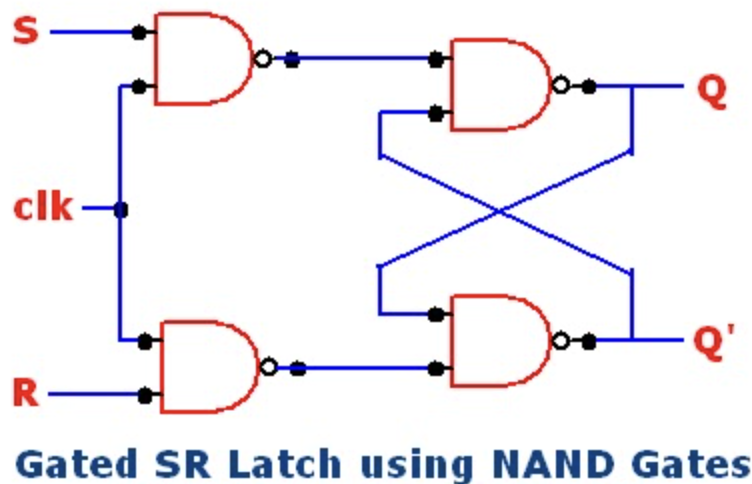
\includegraphics[width=0.5\textwidth]{RS-with-NAND.png}
        \centering
        \caption{Gated SR latch using NAND}
    \end{figure}
\end{definition}

\begin{definition}[Gated D-Latch]
    We can set $D = S = \overline{R}$, so we would prevent $S = R = 1$. So when the clock is HI, $Q$ tracks $D$ (a.k.a. Transparent Mode), and when clock is high, it won't store (a.k.a. Opaque Mode). The truth table is shown as follows:
    \begin{table}[h!]
        \centering
        \begin{tabular}{|c|c||c|}
            \hline
            CLK & $D$ & $Q(t+1)$ \\
            \hline
            0 & X & $Q(t)$ \\
            1 & 0 & 0 \\
            1 & 1 & 1 \\ 
            \hline
        \end{tabular}
        \caption{Truth Table for Gated D Latch}
        \label{tab:gated_d_latch_truth_table}
    \end{table}

    The Verilog implementation is as follows:
    \begin{verbatim}
    module d_latch(input logic D, CLK,
                   output logic Q);
        always_latch begin // this is new in SystemVerilog, 
        // dont write else in always_latch 
            if (CLK) // Transparent mode
                Q = D;
        end
    endmodule
    \end{verbatim}
\end{definition}

\paragraph{Equivalence with a mux} If we feed back the output of a mux back to one of the input, this is essentially a gated D latch with the SW as CLK and the input is the D.

\begin{definition}[D-Flip Flops (Registors)]
    A D flip-flop is a type of flip-flop that captures the value of the D input at a specific portion of the clock cycle (rising edge) and holds that value until the next clock cycle. It is done by chaining the output of a D latch to the input of another D-latch. While the second D-latch recognizes the CLK, and the first one recognizes $\overline{\text{CLK}}$.

    The verilog implementation is as follows:
    \begin{verbatim}
    module d_ff(input logic D, CLK,
                output logic Q);
        always_ff @(posedge CLK) begin
            Q <= D; // Non-blocking assignment
        end
    endmodule
    \end{verbatim}
    \verb|postedge| is a keyword used to create a positive edge-triggered FF. We use $<= $ instead of $= $ because we want to use non-blocking assignment. This is because in a sequential circuit, all the FFs are triggered at the same time, and we want to make sure that the value of Q is updated only after all the FFs have been evaluated.
\end{definition}

\begin{definition}[8-Bit Register]
    An 8-bit register is a digital storage device that can hold 8 bits of binary data. It is typically implemented using a series of D flip-flops, where each flip-flop stores one bit of data. The register has a clock input (CLK) that controls when the data is loaded into the register, and an enable input (EN) that determines whether the register should load new data or retain its current value. When EN is high (1), the register loads the data present on the D input into the flip-flops on the rising edge of the clock. When EN is low (0), the register retains its current value regardless of changes on the D input.

    The Verilog implementation is as follows:
    \begin{verbatim}
    module register8(input logic [7:0] D,
                     input logic CLK, EN,
                     output logic [7:0] Q);
        always_ff @(posedge CLK) begin
            if (EN)
                Q <= D; // Load new data
            // else retain old data
        end
    endmodule
    \end{verbatim}
    
\end{definition}

\paragraph{Resets} We have two types of rests to reset the FF to a known state:
\begin{itemize}
    \item \textbf{Synchronous reset:} Active only on the clock edge. If reset = 1 (or resetn = 0) at the triggering edge the flip‑flop is forced to the predefined state (usually 0); otherwise it captures D.
    \item \textbf{Asynchronous reset:} Active immediately when asserted, forcing the flip‑flop to the predefined state (usually 0) regardless of the clock; normal edge‑triggered operation resumes when deasserted.
\end{itemize}
\begin{definition}[Synchronous Reset D-FF]
    The Verilog implementation is as follows:
    \begin{verbatim}
    module d_ff_sync_reset(input logic D, CLK, RSTn,
                           output logic Q);
        always_ff @(posedge CLK) begin
            if (RSTn == 1'b0)
                Q <= 1'b0; // Reset to 0
            else
                Q <= D; // Normal operation
        end
    endmodule
    \end{verbatim}
    
\end{definition}

\begin{definition}[Asynchronous Reset D-FF]
    The Verilog implementation is as follows:
    \begin{verbatim}
    module d_ff_async_reset(input logic D, CLK, RSTn,
                            output logic Q);
        always_ff @(posedge CLK or negedge RSTn) begin
            if (RSTn == 1'b0)
                Q <= 1'b0; // Reset to 0
            else
                Q <= D; // Normal operation
        end
    endmodule
    \end{verbatim}
\end{definition}

\paragraph{Enable Inputs} We can add an enable input to a D-FF by adding a mux before the D input. It determines whether data is loaded on the clock edge or the old data is retained. If the enable input is high (1), the data on the D input is loaded into the flip-flop on the rising edge of the clock. If the enable input is low (0), there would be a feedback signal going into the mux, so the old data is retained.
\begin{definition}[Counters]
    To count binary numbers, we have the follow truth table:
    \begin{table}[h!]
        \centering
        \begin{tabular}{|c|c|}
            \hline
            CLK Cycle & Binary Count (Q2 Q1 Q0) \\
            \hline
            0 & 000 \\
            1 & 001 \\
            2 & 010 \\
            3 & 011 \\
            4 & 100 \\
            5 & 101 \\
            6 & 110 \\
            7 & 111 \\
            \hline
        \end{tabular}
        \caption{Truth Table for a 3-bit Counter}
        \label{tab:3_bit_counter_truth_table}
    \end{table}
    From the truth table, we can derive the following rules:
    \begin{itemize}
        \item $Q_0$ toggles every clock cycle.
        $$
        Q_0(t+1) = Q_0(t) \oplus 1
        $$
        \item $Q_1$ toggles when $Q_0$ is 1.
        $$
        Q_1(t+1) = Q_1(t) \oplus Q_0(t)
        $$
        \item $Q_2$ toggles when $Q_1$ and $Q_0$ are both 1.
        $$
        Q_2(t+1) = Q_2(t) \oplus (Q_1(t) Q_0(t))
        $$
    \end{itemize}
    We call this a TQ flip-flop, where T stands for toggle. It is done by connecting the Q output back, to a new XOR gate. The input of that XOR gate is Q and T. And the XOR gate output is connected to the D input of a D-FF. The Verilog implementation is as follows:
    \begin{verbatim}
    module counter3(input logic CLK, RSTn,
                    output logic [3:0] Q);
        always_ff @(posedge CLK or negedge RSTn) begin
            if (RSTn == 1'b0)
                Q <= 4'b0000;
            else begin
                Q[0] <= Q[0] ^ 1'b1; // Toggle Q0
                Q[1] <= Q[1] ^ Q[0]; // Toggle Q1
                Q[2] <= Q[2] ^ (Q[1] & Q[0]); // Toggle Q2
                Q[3] <= Q[3] ^ (Q[2] & Q[1] & Q[0]); // Toggle Q3
            end
        end
    endmodule
    \end{verbatim}
\end{definition}

\begin{example}[Clock Reduction]
    Suppose we want to reduce a 1Mhz clock to a 1Hz clock. We can use a 20-bit counter to achieve this. Since $2^{20} = 1,048,576$, which is slightly more than 1 million, we can use the most significant bit (MSB) of the counter as the output clock. The MSB will toggle every $2^{19}$ clock cycles, which is approximately 1 second when the input clock is 1MHz. The Verilog implementation is as follows:
    \begin{verbatim}
    module clock_divider(input logic CLK_1MHZ, RSTn,
                         output logic CLK_1HZ);
        logic [19:0] counter; // 20-bit counter     
        always_ff @(posedge CLK_1MHZ or negedge RSTn) begin
            if (RSTn == 1'b0)
                counter <= 20'b0;
            else
                counter <= counter + 1; // Increment counter
        end
        assign CLK_1HZ = counter[19]; // MSB as 1Hz clock
    endmodule
    \end{verbatim}

    In a real hardware implementation, we would feed the bit to a d flip-flop, and that would create the rising and falling edge signals.
\end{example}

\subsection{Optimizations}

\begin{definition}[Karnaugh Map (K-Map)]
    A Karnaugh map (K-map) is a graphical representation of a truth table that is used to simplify boolean algebra expressions. It is a grid-like structure that organizes the minterms of a boolean function in such a way that adjacent cells differ by only one variable. By grouping adjacent cells that contain 1s, we can identify common factors and simplify the boolean expression.

    The K-map for a 3-variable function is shown below:
    \begin{figure}[h!]
        \centering
        \begin{tabular}{c|c|c|c|c}
            & \multicolumn{4}{c}{BC} \\
            \cline{2-5}
            A & 00 & 01 & 11 & 10 \\
            \hline
            0 & m0 & m1 & m3 & m2 \\
            1 & m4 & m5 & m7 & m6 \\
        \end{tabular}
        \caption{3-Variable Karnaugh Map}
        \label{fig:3_variable_karnaugh_map}
    \end{figure}

    The K-map for a 4-variable function is shown below:
    \begin{figure}[h!]
        \centering
        \begin{tabular}{c|c|c|c|c|c}
            & \multicolumn{4}{c}{CD} \\
            \cline{2-5}
            AB & 00 & 01 & 11 & 10 \\
            \hline
            00 & m0 & m1 & m3 & m2 \\
            01 & m4 & m5 & m7 & m6 \\
            11 & m12 & m13 & m15 & m14 \\
            10 & m8 & m9 & m11 & m10 \\
        \end{tabular}
        \caption{4-Variable Karnaugh Map}
        \label{fig:4_variable_karnaugh_map}
    \end{figure}

    The following rules are used to group the minterms in a K-map:
    \begin{itemize}
        \item Groups must contain only 1s.
        \item Groups must be rectangular and contain $2^n$ cells (where n is a non-negative integer).
        \item Groups can wrap around the edges of the K-map.
        \item Each group should be as large as possible.
        \item Each 1 in the K-map should be covered by at least one group.
    \end{itemize}
    By following these rules, we can create groups of 1s in the K-map and simplify the boolean expression accordingly.
    
\end{definition}

\begin{example}
    Suppose we have the following truth table:
    \begin{table}[h!]
        \centering
        \begin{tabular}{|c|c|c||c|}
            \hline
            A & B & C & F \\
            \hline
            0 & 0 & 0 & 0 \\
            0 & 0 & 1 & 1 \\
            0 & 1 & 0 & 1 \\
            0 & 1 & 1 & 1 \\
            1 & 0 & 0 & 0 \\
            1 & 0 & 1 & 1 \\
            1 & 1 & 0 & 1 \\
            1 & 1 & 1 & 1 \\
            \hline
        \end{tabular}
        \caption{Truth Table for Example}
        \label{tab:example_truth_table}
    \end{table}
    We can derive the following minterms from the truth table:
    $$
    F(A,B,C) = m_1 + m_2 + m_3 + m_5 + m_6 + m_7
    $$
    The K-map for the function is shown below:
    \begin{figure}[h!]
        \centering
        \begin{tabular}{c|c|c|c|c}
            & \multicolumn{4}{c}{BC} \\
            \cline{2-5}
            A & 00 & 01 & 11 & 10 \\
            \hline
            0 & 0 & 1 & 1 & 1 \\
            1 & 0 & 1 & 1 & 1 \\
        \end{tabular}
        \caption{Karnaugh Map for Example}
        \label{fig:example_karnaugh_map}
    \end{figure}
    We can group the minterms as follows:
    \begin{itemize}
        \item Group of four covering $m_2, m_3, m_6, m_7$: This group corresponds to $B = 1$ (since B is constant in this group). So this group simplifies to $B$.
        \item Group of two covering $m_1, m_5$: This group corresponds to $A = 0$ and $C = 1$ (since A and C are constant in this group). So this group simplifies to $\overline{A}C$.
    \end{itemize}
    Therefore, the simplified boolean expression is:
    $$
    F(A,B,C) = B + \overline{A}C
    $$
\end{example}

\begin{definition}[Don't Care Conditions]
    In some cases, certain input combinations may never occur or their output values are irrelevant to the overall function. These input combinations are referred to as "don't care" conditions and are typically represented by an "X" in the truth table. When simplifying a boolean expression using a K-map, we can treat these "don't care" conditions as either 0 or 1, whichever leads to a simpler expression. This flexibility can help in creating larger groups of 1s in the K-map, leading to a more simplified boolean expression.
    
\end{definition}
\begin{example}[Don't Care Conditions]
    Suppose we have the following truth table with don't care conditions:
    \begin{table}[h!]
        \centering
        \begin{tabular}{|c|c|c||c|}
            \hline
            A & B & C & F \\
            \hline
            0 & 0 & 0 & 0 \\
            0 & 0 & 1 & 1 \\
            0 & 1 & 0 & X \\
            0 & 1 & 1 & 1 \\
            1 & 0 & 0 & 0 \\
            1 & 0 & 1 & X \\
            1 & 1 & 0 & 1 \\
            1 & 1 & 1 & 1 \\
            \hline
        \end{tabular}
        \caption{Truth Table with Don't Care Conditions}
        \label{tab:example_dont_care_truth_table}
    \end{table}
    We can derive the following minterms from the truth table:
    $$
    F(A,B,C) = m_1 + m_3 + m_6 + m_7
    $$
    The K-map for the function is shown below:
    \begin{figure}[h!]
        \centering
        \begin{tabular}{c|c|c|c|c}
            & \multicolumn{4}{c}{BC} \\
            \cline{2-5}
            A & 00 & 01 & 11 & 10 \\
            \hline
            0 & 0 & X & 1 & X \\
            1 & 0 & X & 1 & X \\
        \end{tabular}
        \caption{Karnaugh Map with Don't Care Conditions}
        \label{fig:example_dont_care_karnaugh_map}
    \end{figure}
    We can group the minterms as follows:
    \begin{itemize}
        \item Group of four covering $m_3, m_7$ and the don't care conditions: This group corresponds to $C = 1$ (since C is constant in this group). So this group simplifies to $C$.
        \item Group of two covering $m_1$: This group corresponds to $A = 0$ and $B = 0$ (since A and B are constant in this group). So this group simplifies to $\overline{A}\overline{B}$.
    \end{itemize}
    Therefore, the simplified boolean expression is:
    $$
    F(A,B,C) = C + \overline{A}\overline{B}
    $$
\end{example}

\paragraph{Gray Code}
Gray code is a binary numeral system where two successive values differ in only one bit. This property makes Gray code useful in minimizing errors in digital systems, particularly in applications like rotary encoders and digital communication.
The following table shows the 3-bit binary and Gray code representations:
\begin{table}[h!]
    \centering
    \begin{tabular}{|c|c|}
        \hline
        Binary & Gray Code \\
        \hline
        000 & 000 \\
        001 & 001 \\
        010 & 011 \\
        011 & 010 \\
        100 & 110 \\
        101 & 111 \\
        110 & 101 \\
        111 & 100 \\
        \hline
    \end{tabular}
    \caption{3-bit Binary and Gray Code Representations}
    \label{tab:3_bit_binary_gray_code}
\end{table}
\paragraph{Terminologies} For a K-map, we have the following terminologies:
\begin{itemize}
    \item \textbf{Implicant:} A product term (AND term) that can be used to cover one or more minterms in the K-map.
    \item \textbf{Prime Implicant:} An implicant that cannot be combined with any other implicant to form a larger implicant. In other words, it is an implicant that covers the maximum number of minterms possible.
    \item \textbf{Essential Prime Implicant:} A prime implicant that covers at least one minterm that is not covered by any other prime implicant. In other words, it is a prime implicant that is necessary to cover all the minterms in the K-map.
    \item \textbf{Cover:} A set of implicants that together cover all the minterms in the K-map.
\end{itemize}

\begin{example}[Implicant and Prime Implicant]
    Consider the following K-map:
    \begin{figure}[h!]
        \centering
        \begin{tabular}{c|c|c|c|c}
            & \multicolumn{4}{c}{BC} \\
            \cline{2-5}
            A & 00 & 01 & 11 & 10 \\
            \hline
            0 & 1 & 1 & 0 & 0 \\
            1 & 1 & 1 & 1 & 0 \\
        \end{tabular}
        \caption{Karnaugh Map for Example}
        \label{fig:example_karnaugh_map_implicant}
    \end{figure}
    We can identify the following implicants:
    \begin{itemize}
        \item $A'B'$ covering minterms $m_0, m_1$
        \item $A'B$ covering minterms $m_2, m_3$
        \item $AB'$ covering minterms $m_4, m_5$
        \item $AB$ covering minterms $m_6, m_7$
        \item $B$ covering minterms $m_2, m_3, m_6, m_7$
        \item $A$ covering minterms $m_4, m_5, m_6, m_7$
    \end{itemize}
    The prime implicants are:
    \begin{itemize}
        \item $A'B'$ (cannot be combined with any other implicant)
        \item $B$ (cannot be combined with any other implicant)
        \item $A$ (cannot be combined with any other implicant)
    \end{itemize}
    The essential prime implicants are:
    \begin{itemize}
        \item $A'B'$ (covers minterm $m_0$ which is not covered by any other prime implicant)
        \item $B$ (covers minterms $m_2, m_3$ which are not covered by any other prime implicant)
        \item $A$ (covers minterms $m_4, m_5$ which are not covered by any other prime implicant)
    \end{itemize}
    Therefore, the cover of the K-map is:
    $$
    F(A,B,C) = A'B' + B + A
    $$
\end{example}

\begin{example}
    Let $f(x_1, x_2, x_3, x_4) = \sum m(2, 4, 5, 8, 10, 11, 12, 13, 15)$ be a function represented by the following K-map:
    % up : x_1 x_2, left: x_3 x_4
    \begin{figure}[h!]
        \centering
        \begin{tabular}{c|c|c|c|c}
            & \multicolumn{4}{c}{$x_1 x_2$} \\
            \cline{2-5}
            $x_3 x_4$ & 00 & 01 & 11 & 10 \\
            \hline
            00 & 0 & 1 & 1 & 1 \\
            01 & 0 & 1 & 1 & 0 \\
            11 & 0 & 0 & 1 & 1 \\
            10 & 1 & 0 & 0 & 1 \\   
        \end{tabular}
        \caption{Karnaugh Map for Example}
        \label{fig:example_karnaugh_map_dont_care}
    \end{figure}

\end{example}



\paragraph{Procedure to fine the minimum cost cover}
\begin{enumerate}
    \item Find all prime implicants.
    \item Identify all essential prime implicants (EPIs) and include them in the cover.
    \item Remove all minterms covered by the EPIs from the K-map.
    \item Check and inspect whether it is the minimum cost cover. 
\end{enumerate}


\begin{definition}[K-Maps with Maxterm]
    We can also use K-maps to simplify boolean expressions represented by maxterms. The procedure is similar to that of minterms, but instead of grouping 1s, we group 0s. The following rules are used to group the maxterms in a K-map:
    \begin{itemize}
        \item Groups must contain only 0s.
        \item Groups must be rectangular and contain $2^n$ cells (where n is a non-negative integer).
        \item Groups can wrap around the edges of the K-map.
        \item Each group should be as large as possible.
        \item Each 0 in the K-map should be covered by at least one group.
    \end{itemize}
    By following these rules, we can create groups of 0s in the K-map and
\end{definition}


\section{Finite State Machines (FSM)}
\begin{definition}[State Diagram]
    A state diagram is a graphical representation of a finite state machine (FSM) that illustrates the states, transitions, inputs, and outputs of the system. It consists of nodes (representing states) and directed edges (representing transitions between states). Each edge is typically labeled with the input condition that triggers the transition and may also include the output associated with that transition.

    State diagrams are used to visualize the behavior of sequential systems, making it easier to understand how the system responds to different inputs and how it transitions between various states over time.
\end{definition}

\begin{example}
    Cosnider a circult that detect the input sequance $w=$`101' using a FSM. The state diagram is shown below:
    \begin{figure}[h!]
        \centering
        \begin{tikzpicture}[node distance=2cm, on grid, auto]
            % Nodes
            \node[state, initial] (S0) {S0};
            \node[state] (S1) [right=of S0] {S1};
            \node[state] (S2) [right=of S1] {S2};
            \node[state, accepting] (S3) [right=of S2] {S3};    
            % Edges
            \path[->]
                (S0) edge [loop above] node {0/0} ()
                     edge node {1/0} (S1)
                (S1) edge node {0/0} (S2)
                     edge [loop above] node {1/0} ()
                (S2) edge node {1/1} (S3)
                     edge [bend left] node {0/0} (S0)
                (S3) edge [bend left] node {0/0} (S2)
                     edge [bend left] node {1/0} (S1);
        \end{tikzpicture}
        \caption{State Diagram for FSM that detects `101'}
        \label{fig:fsm_state_diagram}
    \end{figure}
    The FSM has four states: S0, S1, S2, and S3. The initial state is S0, and the accepting state is S3. The transitions between states are labeled with the input/output pairs. For example, from state S0, if the input is 1, the FSM transitions to state S1 and outputs 0. The FSM detects the sequence `101' and outputs 1 when it reaches state S3.
    
    We can also draw its state table as follows:
    \begin{table}[h!]
        \centering
        \begin{tabular}{|c|cc|c|}
            \hline
            Curreent State & $w=0$ & $w=1$ & Output \\
            \hline
            S0 & S0 & S1 & 0 \\
            S1 & S2 & S1 & 0 \\
            S2 & S0 & S3 & 0 \\
            S3 & S2 & S1 & 1 \\
            \hline
        \end{tabular}
        \caption{State Table for FSM that detects `101'}
        \label{tab:fsm_state_table}
    \end{table}

    Then, we would assign the states. First the circuit has 4 states, so we need at least 2 flip-flops $y_2$, $y_1$ to represent the states. We can assign the states as follows:
    \begin{itemize}
        \item S0 = 00, $y_2 y_1$
        \item S1 = 01, $y_2 \overline{y_1}$
        \item S2 = 10, $\overline{y_2} y_1$
        \item S3 = 11, $\overline{y_2} \overline{y_1}$
    \end{itemize}
    Then, we can derive the following state transition table:

    \begin{table}[h!]
        \centering
        \begin{tabular}{|c|cc|c|}
            \hline
            Current State ($y_2 y_1$) & $w=0$ & $w=1$ & Output \\
            \hline
            00 & 00 & 01 & 0 \\
            01 & 10 & 01 & 0 \\
            10 & 00 & 11 & 0 \\
            11 & 10 & 01 & 1 \\
            \hline
        \end{tabular}
        \caption{State Transition Table for FSM that detects `101'}
        \label{tab:fsm_state_transition_table}
    \end{table}

    From the state transition table, we can synthesis the circuit using D flip-flops. Let $Y_2$ and $Y_1$ be the next state of $y_2$ and $y_1$, respectively. We can derive the following equations:
    \begin{itemize}
        \item $Y_1 = w$
        \item $Z = y_2 y_1$
        \item $Y_2 = \overline{w} y_1 + w \overline{y_2} \overline{y_1}$
    \end{itemize}
    
\end{example}

\begin{definition}[Finite State Machine (FSM)]
    A finite state machine (FSM) is a mathematical model of computation used to design both computer programs and sequential logic circuits. It is composed of a finite number of states, transitions between those states, inputs, and outputs. FSMs are used to model the behavior of systems that can be in one of a limited number of states at any given time and can transition from one state to another based on input signals.

    There are two main types of FSMs:
    \begin{itemize}
        \item \textbf{Moore Machine:} In a Moore machine, the outputs depend only on the current state. The output is associated with each state, and it changes only when the state changes.
        \item \textbf{Mealy Machine:} In a Mealy machine, the outputs depend on both the current state and the current inputs. The output can change immediately in response to changes in the input, even if the state remains the same.
    \end{itemize}
\end{definition}
\chapter{Computer Organization and Assembly Language}
\begin{shaded}
\textbf{What is Assembly Language?} We know that we can run C/C++ on any computer (Machine Agnostic), but how does the computer understand C/C++? The answer is the compiler that parse it to assembly through:

\begin{enumerate}
    \item \textbf{Front-end Parser:} The front-end parser would parse the C/C++ code into an intermediate representation (IR), which is a low-level representation of the code that is easier to optimize. The front-end parser would also perform optimizations on the IR, such as loop unrolling, inlining, and dead code elimination.
    \item \textbf{Back-end Parser:} The back-end parser would take the optimized IR and generate assembly code for a specific architectures.
\end{enumerate}
\end{shaded}
The assembly code is then assembled into machine code, which is a series of 0s and 1s that the computer can understand. The assembly would be specific to the architecture of the computer (machine dependent), which is why we have different assembly languages for different architectures (e.g., x86, RISC-V, ARM).
\section{Computer Organization}
\section{Assembly Language}
\end{document}

